Figure~\ref{fig:nondeterminism} shows an example multithreaded program that, because of data races, non-deterministically produces the outputs: ``1,0,'' ``0,1,'' and ``1,1.''  The order of instructions are changed from one execution to the other, resulting in these nondeterministic outputs. Using \dthreads{}, this program will \emph{deterministically} produce the same output ``1,1.'' Although this output can be a undesired one, the fact that results are always reproducible would make it easy for developers to reproduce and locate data races inside parallel programs.

\begin{figure}[h]
{\centering
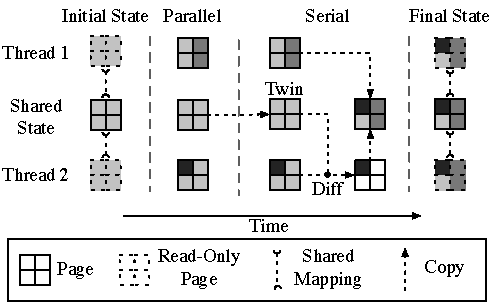
\includegraphics[width=6in]{dthreads/figure/architecture-diagram}
\caption{An overview of \dthreads{} execution.\label{fig:architecture}}
}
\end{figure}

\dthreads{} employs the following mechanisms to ensure the deterministic execution, illustrated by Figure~\ref{fig:architecture}: 

\textbf{Isolated Memory Access:} In \dthreads{}, threads are actually running as separate processes with private and shared views of memory, which is based on the \sheriff{} framework. Because processes have separate address spaces, \dthreads{} can isolate executions of different ``threads.'' \dthreads{} uses this isolation mechanism to control the visibility of memory state, so that updates made by a thread can not be seen by other threads if those updates are not committed explicitly to the shared mapping. By doing this, we guarantee that each ``thread'' can operate independently until synchronization points. Implementations are discussed in depth in Section~\ref{sec:threadsasprocs}.

\textbf{Deterministic Memory Commit:} 
Multithreading programs use shared memory for communication, thus \dthreads{} must make a thread's changes seen by other threads. To guarantee determinism, \dthreads{} should publish updates of different threads in a deterministic order at deterministic points.

\dthreads{} actually commits the changes of a thread to the shared state in sequence at synchronization points. These points includes thread creation and exit; mutex lock and unlock; condition variable wait and signal; posix sigwait and signal; and barrier waits. Commits are ordered using a global token that is passed from one thread to the next; a thread can only commit when it holds the token.  The token-passing protocol is described in Section~\ref{sec:schedule} and the implementation of synchronization primitives is described in Section~\ref{sec:synchronization}.

\dthreads{} relies on the twinning and diffing mechanism to find out local changes of different threads, which has been discussed in Section~\ref{sec:twinning-and-diffing}. 

\textbf{Deterministic Synchronization:}
There is no deterministic guarantee on synchronizations under existing operating systems. Thus, \dthreads{} re-implements the full range of pthreads synchronization primitives and discusses  them in details in Section~\ref{sec:synchronization}. 

\hspace{1em} \\
\noindent
\textbf{Fixing the data race example} \\
About the example program in Figure~\ref{fig:nondeterminism},  \dthreads{} effectively isolates the execution from each thread until it completes, and then orders updates from different threads by thread creation time using a deterministic last-writer-wins protocol.

In the beginning of every execution, thread 1 and thread 2 have the same view of shared state, with a = 0 and b = 0. Since changes by one thread to the value of a or b are not visible to the other until this thread exits, both checks on two threads on line 2 will be true. Thread 1 sets the value of a to 1, and thread 2 sets the value of b to 1. These threads then commit their updates to the shared state and exit, with thread 1 always committing before thread 2. The main thread then should always print ``1, 1'' on every execution.

Determinism not only enables replay-without-recording and replicated executions, but also effectively converts ``Heisenbugs'' into ``Bohr'' bugs, making them reproducible. In addition, \dthreads{} optionally reports any conflicting updates due to racy writes, further simplifying debugging.
